\documentclass[11pt]{article}

\usepackage[margin=1in]{geometry}
\usepackage{amsmath,amssymb,bm}
\usepackage{booktabs}
\usepackage{graphicx}
\usepackage{tikz}
\usepackage[colorlinks=true,linkcolor=blue,urlcolor=blue]{hyperref}

\newcommand{\dlam}{\tfrac{d}{\lambda}}
\newcommand{\pinorm}{\operatorname{pi\_norm}}

\title{SPF: Background, Problem Space, and Approach\\
\large RF emitter localization with two-element software-defined radio arrays}
\author{Project SPF}
\date{\today}

\begin{document}
\maketitle

\begin{abstract}
SPF localizes radio-frequency emitters using pairs of cheap two-antenna
software-defined radios (SDRs) mounted on mobile rovers and on a mechanically
positioned wall array. This document motivates the project, maps the problem
space, and describes the approach: large-scale real-world data collection, a
careful physical model of what a two-element array can and cannot measure, and
learned models plus filtering that recover bearing (and, with multiple
receivers, position) despite ambiguity and hardware imperfection. A dedicated
section walks step by step through the core mathematics: how the phase
difference between two antennas encodes the angle of arrival, where the
ambiguities come from, and how the same forward model powers both the neural
networks' inputs and the dataset-quality audit.
\end{abstract}

\tableofcontents
\clearpage

\section{Motivation}
\label{sec:motivation}

Finding \emph{where a radio transmission is coming from} is a classical problem
with modern urgency: locating a lost drone by its video downlink, finding an
interference source that is degrading a shared band, tracking wildlife tags,
or navigating toward a beacon when GPS is unavailable. Commercial
direction-finding gear solves this with large, calibrated, many-element
antenna arrays and correspondingly large price tags.

SPF starts from the opposite end of the cost spectrum and asks:

\begin{quote}
\emph{How much localization capability can be extracted from the cheapest
possible sensor --- a single pair of antennas attached to a \$100--\$200
software-defined radio --- if we are willing to move the sensor, collect a lot
of real data, and learn the sensor's imperfections instead of engineering them
away?}
\end{quote}

Three observations make this question worth asking.

\paragraph{1. Two antennas are the minimal interferometer.}
A two-element array measures exactly one number per snapshot --- the phase
difference between its channels --- and that number is a (nonlinear,
ambiguous, noisy) function of the emitter bearing
(Section~\ref{sec:math}). Everything the platform will ever know about
direction must be squeezed out of this one degree of freedom, plus motion,
plus time. It is the sharpest possible test bed for ``sensing with learned
models'': the physics is simple enough to write down exactly, yet the
real-world measurement deviates from that physics in ways that are hard to
calibrate by hand (mount rotations, effective antenna spacing, gain-dependent
phase inversions, automatic gain control, multipath).

\paragraph{2. Motion converts ambiguity into information.}
A stationary two-element array cannot distinguish front from back, and for
wide antenna spacing cannot even pin down a unique bearing
(Section~\ref{sec:ambiguity}). But a \emph{moving} receiver-- or a pair of
receivers --- sweeps its ambiguity structure through space; a filter that
accumulates measurements over a trajectory can collapse the ambiguity. This
trades hardware complexity for algorithmic complexity, which is exactly the
trade a learned system should win.

\paragraph{3. Real data beats simulated calibration.}
Early experiments made it clear that the dominant error sources are not
thermal noise but \emph{systematics}: antennas mounted a few millimetres from
their nominal positions, arrays labeled with the wrong spacing, compass biases
that drift between calibration sessions, receiver gain control interacting
with the RF front end. These are properties of each physical rig on each
particular day. SPF therefore treats large-scale, ground-truth-annotated data
collection --- and the auditing of that data
(Section~\ref{sec:audit-approach}) --- as a first-class part of the project,
on equal footing with model architecture.

\section{Problem space}
\label{sec:problem}

\subsection{Task statement}

Given streams of IQ samples from the two RX channels of one or more
two-antenna SDR receivers, each annotated with the receiver's pose (position,
heading) and, at training time, the emitter's ground-truth position, estimate:

\begin{enumerate}
  \item \textbf{Bearing} $\theta$ of the emitter relative to each receiver
        (the \emph{single-radio} problem);
  \item \textbf{Fused bearing / position} using two radios on one platform or
        multiple platforms over time (the \emph{paired} and \emph{filtering}
        problems).
\end{enumerate}

\subsection{Hardware platforms}

\paragraph{Wall array (controlled environment).}
A GRBL-driven 2-axis gantry moves an emitter across a wall while fixed
two-antenna receivers (PlutoSDR class, and later BladeRF~2 on a desk rig)
record. Ground truth is sub-millimetre from the stepper positions. This
platform isolates the RF chain: with essentially perfect geometry, any
residual between predicted and measured phase is a property of radios,
antennas, mounts, and environment --- which is what makes it the reference
platform for the data audit.

\paragraph{Rovers (field environment).}
Skid-steer rovers carry receivers (and one carries the emitter) around a
field; poses come from GPS and compass, so ground-truth bearing error of a few
degrees is intrinsic (3\,m GPS error at 15\,m range is
$\approx 0.2$\,rad). Multiple rovers record simultaneously and their captures
are merged into paired datasets (TX rover $\times$ RX rover).

\paragraph{Radios and signals.}
AD9361-family 2$\times$RX SDRs (PlutoPlus, BladeRF~2) sampling up to
30\,MHz. Emitters are continuous-wave-like beacons (ESP32 ``tone blaster'' on
2.4\,GHz Wi-Fi channels; analog video transmitters at 5.7--5.9\,GHz; sub-GHz
LoRa-class modules at 868/915\,MHz). Configured antenna spacings range from
$d/\lambda \approx 0.21$ to $1.55$ across the fleet --- deliberately including
spacings well past the unambiguous limit of $d/\lambda = 1/2$
(Section~\ref{sec:ambiguity}).

\subsection{What makes it hard}

\begin{description}
  \item[Ambiguity by construction.] Front--back mirror symmetry always;
    grating-lobe aliasing whenever $d/\lambda > 1/2$. The sensor
    \emph{by design} does not determine a unique bearing per snapshot.
  \item[Systematic hardware error.] Mount rotations and mislabeled spacings
    (both have occurred and were later fixed by ``data surgery''), effective
    spacing differing from configured spacing (antenna coupling, connector
    geometry), per-channel LO phase offsets.
  \item[Gain control interactions.] The AD9361 runs fast-attack AGC; gain
    changes of 17--39\,dB occur within datasets, and gain-index changes can
    invert channel polarity at the LNA-bypass boundary --- a $\pi$ phase jump
    in the measurement of interest.
  \item[Intermittent, contested spectrum.] Duty-cycled emitters (burst
    beacons, $\sim$1--3\% airtime in the extreme), other transmitters in-band
    (Wi-Fi, other 5.8\,GHz video links), and sessions with recorded
    interference incidents.
  \item[Label noise on moving platforms.] GPS + compass ground truth is
    itself noisy and era-dependent (compass calibration events shift the bias).
  \item[Scale and drift of the corpus.] Thousands of capture sessions
    collected over $\sim$1.5 years, across hardware revisions, firmware
    versions, frequency bands, and collection sites. Quality is strongly
    era-dependent; some months are systematically bad. Training and evaluating
    on this corpus requires an explicit quality model of the corpus itself.
\end{description}

\subsection{Why not classical array processing alone?}

MUSIC/ESPRIT-style methods assume a calibrated steering model and more
elements than sources. With two elements, one source, uncalibrated mounts, and
gain-dependent polarity, the classical estimate collapses to
$\hat\theta = \arcsin(-\hat\varphi\,\lambda/2\pi d)$ applied to a noisy,
aliased $\hat\varphi$ --- brittle exactly where our data lives. The physics
still matters (it defines the feature space and the audit's forward model),
but the mapping from measured phase statistics to bearing posterior is
learned, and ambiguity resolution is deferred to fusion and filtering.

\section{Signals background: how we get complex numbers out of an antenna}
\label{sec:iq}

The math section ahead manipulates ``complex baseband samples'' as if that
were the obvious thing a radio produces. It is not obvious. This section
motivates it from scratch: what the antenna really measures, why we describe
it with complex numbers, what I/Q means, and precise working definitions of
the terms (narrowband, broadband, window, coherent) used everywhere else.

\subsection{What the antenna actually measures}
\label{sec:antenna}

An antenna is a wire; the only thing it can give the receiver is a
\emph{real} voltage that wiggles in time, $v(t)$. For a 2.412\,GHz emitter
that voltage oscillates 2.4 \emph{billion} times per second. Almost none of
those wiggles are interesting individually --- the information (and, for us,
the geometry) rides on how the wiggle's \emph{strength} and \emph{timing}
drift over microseconds, millions of times slower than the wiggle itself.

Any such signal can be written as
\[
v(t) \;=\; A(t)\,\cos\!\big(2\pi f t + \psi(t)\big),
\]
where $f$ is the \textbf{carrier frequency} (the fast wiggle),
$A(t) \ge 0$ is the \textbf{amplitude} or \textbf{envelope} (how strong the
wiggle currently is), and $\psi(t)$ is the \textbf{phase} (how the wiggle is
currently shifted relative to a perfect clock at frequency $f$). $A$ and
$\psi$ change slowly compared to the carrier; they are ``the signal''. The
pair $(A, \psi)$ is what we actually want, sampled in time.

\subsection{Why complex numbers: one arrow instead of two numbers}

A pair (strength, angle) is naturally a single \emph{arrow} in the plane ---
a complex number:
\[
x(t) \;=\; A(t)\, e^{j\psi(t)}
\qquad\text{(length $=$ amplitude, direction $=$ phase).}
\]
This is not just notation. The two operations radio processing does
constantly become trivial arithmetic on arrows:
\begin{itemize}
  \item \textbf{Delaying} a narrowband signal by $\tau$ rotates its arrow by
        a fixed angle: $x(t-\tau) \approx x(t)\,e^{-j2\pi f \tau}$
        (the envelope barely moves, the carrier phase shifts). Delay ---
        which is geometry --- becomes multiplication.
  \item \textbf{Comparing} two channels becomes one multiplication:
        $x_1 x_0^{*}$ has length $A_1 A_0$ and angle $\psi_1 - \psi_0$. The
        entire two-antenna measurement of Section~\ref{sec:math} is this one
        product.
\end{itemize}
With real cosines both operations are trigonometric-identity soup; with
arrows they are one-liners. That is the whole reason radios use complex
numbers.

\subsection{I/Q: how the hardware extracts the arrow}
\label{sec:iq-demod}

\paragraph{The cast.}
Recall from Section~\ref{sec:antenna} what $v(t)$ is: the \emph{real} voltage
on the antenna wire,
\[
v(t) = A\cos(2\pi f t + \psi),
\]
where $f$ is the carrier ($\sim$2.4 billion wiggles per second), $A$ is how
strong the wave currently is, and $\psi$ is its timing shift relative to a
perfect clock at frequency $f$. ($A$ and $\psi$ do change with time, but a
million times slower than the carrier --- over the few nanoseconds this
derivation cares about they are constants.) The receiver wants $A$ and $\psi$
but can only measure $v(t)$, in which they are tangled up inside the cosine.
Three hardware pieces untangle them:
\begin{itemize}
  \item the \textbf{local oscillator (LO)}: the radio's own clean internal
        tone at the carrier frequency --- it can generate $\cos(2\pi f t)$ and
        (by delaying a quarter cycle) $\sin(2\pi f t)$;
  \item a \textbf{mixer}: a circuit that literally multiplies two voltages;
  \item a \textbf{low-pass filter}: a circuit that averages away anything
        wiggling faster than some cutoff, keeping only slow variations.
\end{itemize}

\paragraph{The one identity that does all the work.}
Multiplying two cosines produces the sum and difference of their angles ---
the product-to-sum identity from trigonometry:
\[
2\cos(a)\cos(b) = \cos(a-b) + \cos(a+b),
\qquad
2\cos(a)\sin(b) = \sin(a+b) - \sin(a-b).
\]
The trick of the whole receiver: choose $b$ = the LO's angle $2\pi f t$, and
$a$ = the signal's angle $2\pi f t + \psi$. Then the \emph{difference}
$a - b = \psi$ --- the fast carrier subtracts out, leaving exactly the
quantity we want --- while the \emph{sum} $a + b = 4\pi f t + \psi$ wiggles at
twice the carrier and can be filtered away.

\paragraph{I branch, line by line.}
Multiply the antenna voltage by twice the LO cosine and apply the first
identity with $a = 2\pi f t + \psi$, $b = 2\pi f t$:
\begin{align*}
v(t)\cdot 2\cos(2\pi f t)
  &= 2A\cos(2\pi f t + \psi)\cos(2\pi f t)\\
  &= A\cos(\underbrace{\psi}_{a-b})
     \;+\; \underbrace{A\cos(4\pi f t + \psi)}_{a+b:\ \text{wiggles at }2f}
  \;\xrightarrow{\text{low-pass}}\; I = A\cos\psi .
\end{align*}
The second term oscillates at $2f \approx 4.8$\,GHz --- averaging over even a
few carrier cycles kills it; the first term is constant (on carrier
timescales) and sails through the filter.

\paragraph{Q branch, line by line.}
Same signal, multiplied by the quarter-cycle-shifted copy of the LO, using
the second identity:
\begin{align*}
v(t)\cdot \big(-2\sin(2\pi f t)\big)
  &= -2A\cos(2\pi f t + \psi)\sin(2\pi f t)\\
  &= A\sin(\underbrace{\psi}_{a-b})
     \;-\; \underbrace{A\sin(4\pi f t + \psi)}_{\text{at }2f}
  \;\xrightarrow{\text{low-pass}}\; Q = A\sin\psi .
\end{align*}
(The minus sign on the LO copy is chosen so the surviving term comes out as
$+A\sin\psi$.)

\paragraph{Why two branches are necessary.}
One branch alone gives $I = A\cos\psi$ --- a single number that hopelessly
mixes strength and timing: $I = 0.5$ could be a strong signal at
$\psi = 60^\circ$ or a weak one at $\psi = 0^\circ$, and $\psi$ and $-\psi$
are indistinguishable. The arrow lives in a plane; you need its shadow along
\emph{two} perpendicular directions to pin it down. $I$ and $Q$ are exactly
those two shadows, and together they reconstruct it uniquely:
\[
x = I + jQ = A\cos\psi + jA\sin\psi = A e^{j\psi},
\qquad
A = \sqrt{I^2 + Q^2}, \quad \psi = \operatorname{atan2}(Q, I).
\]
Worked example: $A = 1$, $\psi = 60^\circ$ gives $I = 0.5$, $Q = 0.866$ ---
the point $(0.5, 0.866)$, an arrow of length 1 at $60^\circ$.

\textbf{I} is the \emph{in-phase} component (relative to the LO cosine),
\textbf{Q} the \emph{quadrature} (90$^\circ$-shifted) component. The SDR
digitizes both at the \textbf{sample rate} $f_s$ (up to 30\,MHz here),
producing the complex \textbf{baseband} stream $x[n]$ used everywhere in this
document. ``Baseband'' means the carrier has been divided out: a pure
unmodulated carrier at exactly the LO frequency becomes a \emph{constant}
arrow.

\paragraph{When the LO is not exactly the carrier.}
Everything above assumed the LO frequency equals $f$. In reality the radio is
tuned to $f_{\mathrm{LO}} = f - f_{\mathrm{IF}}$ (deliberately, plus crystal
error), and redoing the derivation with $b = 2\pi f_{\mathrm{LO}} t$ gives
$a - b = 2\pi f_{\mathrm{IF}} t + \psi$: the surviving slow term is not a
constant but a slow rotation at the \emph{intermediate frequency}
$f_{\mathrm{IF}} = f - f_{\mathrm{LO}}$. The arrow spins at $f_{\mathrm{IF}}$
turns per second. This is why IF placement matters so much for data quality
(the dataset-quality report's tone-at-DC analysis): $f_{\mathrm{IF}} \approx 0$
parks the spinning arrow on top of the receiver's DC machinery, while a
healthy offset keeps it clear --- and since both antennas share one LO, the
spin is common to both channels and cancels in the phase difference.

Two hardware facts matter enormously for SPF:
\begin{itemize}
  \item \textbf{Both RX channels of the AD9361 share one LO.} The arbitrary
        LO phase appears identically in $\psi_0$ and $\psi_1$ and cancels in
        $x_1 x_0^{*}$. This is why the \emph{inter-channel phase difference}
        is physically meaningful and stable, even across signal bursts, while
        the \emph{absolute} phase of either channel alone is meaningless.
  \item \textbf{The LO is never exactly the emitter's carrier.} A small
        frequency offset makes the arrow rotate slowly (``spin''); it is
        common to both channels and cancels in the difference, but it is why
        single-channel phase drifts and must be detrended in some analyses.
\end{itemize}

\paragraph{Remark: I/Q as value and derivative (phase space).}
There is a physicist's way to see all of this at once. At any instant, the
waveform's \emph{value} is $v = A\cos\theta$ and its \emph{scaled
derivative} is $-v'/(2\pi f) = A\sin\theta$ (differentiating a cosine
yields the sine; the carrier dominates the slope). So (value, derivative) are
the same two numbers as (I, Q), just measured in the lab frame at the total
angle $\theta = 2\pi f t + \psi$; the LO's rotating frame subtracts the
known carrier ramp and freezes the arrow at $\psi$. Deeper still: a sinusoid
is a harmonic oscillator, whose state space is exactly two-dimensional ---
(position, velocity), $(A, \psi)$, and $(I, Q)$ are three coordinates for the
same state, which is why two branches are necessary and sufficient (and why
$I$ and $Q$ are called \emph{quadratures}, the oscillator's $x$ and $p$).
The hardware mixes rather than differentiates for practical reasons only: a
differentiator at 2.4\,GHz would need sub-cycle timing, amplifies noise
$\propto$ frequency, and reads one instant --- while mixer + low-pass
measures the same two numbers averaged over thousands of carrier cycles.

\subsection{Term definitions used throughout}
\label{sec:terms}

\begin{description}
  \item[Carrier / baseband.] The carrier is the fast oscillation at $f$;
        baseband is the slow complex signal $x(t)$ left after the carrier is
        mixed out.
  \item[Bandwidth $B$.] How fast the arrow moves: the width of the frequency
        band occupied by $A(t)e^{j\psi(t)}$. A pure tone has $B \to 0$; a
        20\,MHz Wi-Fi packet has $B = 20$\,MHz.
  \item[Narrowband (for our purposes).] Two conditions, both comfortably true
        in SPF: (i) $B \ll f$ (the signal is a thin slice around the
        carrier), and (ii) --- the one that matters for arrays ---
        $B\,\tau \ll 1$, where $\tau \le d/c$ is the inter-antenna delay: the
        envelope does not change in the $\sim$0.2\,ns it takes the wave to
        cross the array, so both antennas see \emph{the same} $A$ and $\psi$
        and differ only by the geometric rotation $e^{-j2\pi f\tau}$. Even
        Wi-Fi ($B\tau \approx 4\times10^{-3}$) passes easily.
  \item[Broadband / wideband.] $B\tau$ not small, or $B/f$ large: different
        frequency components inside the signal have different wavelengths,
        hence \emph{different} inter-antenna phase shifts --- a single
        $\varphi$ no longer summarizes the geometry and processing must split
        the band (e.g.\ per-subcarrier). SPF's beacons do not operate here,
        but strong wideband interferers do.
  \item[Window.] A contiguous run of $N$ samples treated as one measurement
        unit; SPF computes phase/beamformer statistics per window, many
        windows per snapshot.
  \item[Snapshot / session.] A snapshot is one capture buffer with one
        ground-truth pose; a session (dataset) is the full recorded
        trajectory of snapshots.
  \item[Coherent vs.\ incoherent combining.] Coherent: add the complex
        arrows, \emph{then} take magnitude/angle --- signals aligned in phase
        reinforce ($N$ arrows of unit length aligned give length $N$; random
        phases give $\sim\sqrt{N}$), so SNR grows with window length.
        Incoherent: add magnitudes or powers, discarding phase --- robust
        when phase is unstable, but no phase gain. The coherent sum
        $\sum x_1 x_0^{*}$ of Section~\ref{sec:estimation} is the coherent
        combine of the \emph{difference} arrows.
  \item[SNR.] Signal-to-noise power ratio within the processed band; window
        statistics turn per-sample SNR into per-window estimate quality.
\end{description}

With this vocabulary, the math section can be read literally: every
``complex baseband sample'' is an I/Q arrow, every phase difference is an
angle between two arrows sharing one clock, and every ``narrowband''
invocation is the statement $B\tau \ll 1$ justified above.

\section{The mathematics: from phase difference to angle}
\label{sec:math}

This section is deliberately slow. Everything SPF does --- the beamformer
features fed to the networks, the symmetry constraints in training, the
particle filter's measurement model, and the dataset audit's forward model ---
is a consequence of one small piece of geometry, so it pays to derive it once,
carefully, with signs and conventions pinned down.

\subsection{Setup and conventions}
\label{sec:setup}

Two receive antennas $A_0$ and $A_1$ are separated by a baseline of length
$d$ (metres). Place the midpoint of the baseline at the origin, with the
baseline along the $x$-axis:
\[
A_0 = \left(+\tfrac{d}{2},\, 0\right), \qquad
A_1 = \left(-\tfrac{d}{2},\, 0\right).
\]
The \emph{boresight} (broadside) direction is the $+y$-axis, perpendicular to
the baseline. An emitter lies at range $R$ in direction $\theta$, where
$\theta$ is measured \emph{from boresight}, positive toward $+x$ (toward
$A_0$):
\[
E = (R\sin\theta,\; R\cos\theta).
\]
The emitter transmits a narrowband signal at carrier frequency $f$ with
wavelength $\lambda = c/f$ ($c$ the speed of light). At 2.412\,GHz,
$\lambda = 12.4$\,cm; at 5.766\,GHz, $\lambda = 5.2$\,cm; at 915\,MHz,
$\lambda = 32.8$\,cm.

\begin{figure}[ht]
\centering
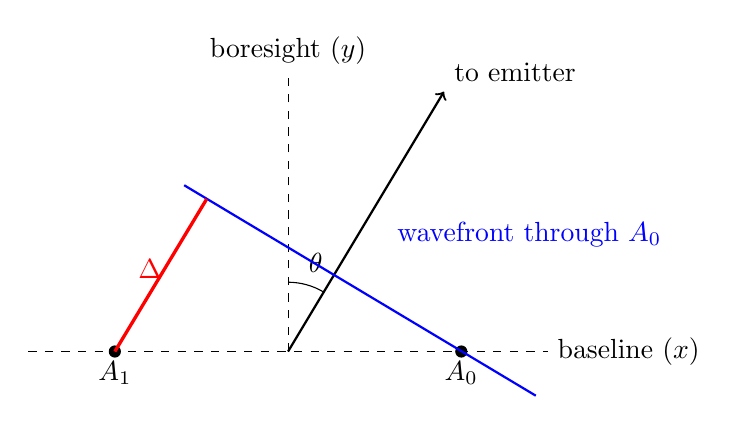
\begin{tikzpicture}[scale=1.1]
  % geometry precomputed for arrival direction u = (1.8,3.0)/|.| = (0.5145,0.8575),
  % i.e. theta = 31.0 deg east of boresight
  % antennas
  \fill (2,0) circle (2pt) node[below] {$A_0$};
  \fill (-2,0) circle (2pt) node[below] {$A_1$};
  \draw[dashed] (-3,0) -- (3,0) node[right] {baseline ($x$)};
  \draw[dashed] (0,0) -- (0,3.2) node[above] {boresight ($y$)};
  % arrival direction
  \draw[->,thick] (0,0) -- (1.8,3.0) node[above right] {to emitter};
  \draw (0,0.8) arc[start angle=90, end angle=59, radius=0.8];
  \node at (0.32,1.02) {$\theta$};
  % wavefront through A0: line through (2,0) perpendicular to u
  \draw[thick,blue] (2.86,-0.51) -- (-1.20,1.92);
  \node[blue, right] at (1.15,1.35) {wavefront through $A_0$};
  % extra path: A1 to its projection F = A1 + ((A0-A1).u) u = (-0.94,1.76)
  \draw[very thick,red] (-2,0) -- (-0.94,1.76);
  \node[red, left] at (-1.35,0.95) {$\Delta$};
\end{tikzpicture}
\caption{Far-field geometry. The wavefront (perpendicular to the arrival
direction) reaches $A_0$ first; $A_1$ waits for the wave to cover the extra
red path $\Delta = d\sin\theta$.}
\label{fig:geometry}
\end{figure}

\subsection{Step 1: the far-field assumption}
\label{sec:farfield}

Exactly, the two path lengths are $\lVert E - A_0\rVert$ and
$\lVert E - A_1\rVert$. Expanding $\lVert E - A_{0,1}\rVert$ in powers of
$d/R$:
\[
\lVert E - A_{0,1}\rVert
  = R \mp \tfrac{d}{2}\sin\theta
    + \frac{d^2\cos^2\theta}{8R} + O\!\left(\frac{d^3}{R^2}\right).
\]
The first-order term is the plane-wave (far-field) result; the quadratic term
is the near-field (wavefront curvature) correction. Its phase contribution is
$2\pi/\lambda \cdot d^2/(8R)$ at worst. Plugging in wall-array numbers
($d = 5$\,cm, $R = 0.9$\,m, $\lambda = 12.4$\,cm): the correction is
$\approx 0.018$\,rad --- negligible against measured phase noise, and it was
explicitly ruled out as a residual source in the audit. From here on we work
in the far field: incoming wavefronts are planes perpendicular to the arrival
direction.

\subsection{Step 2: path-length difference}
\label{sec:pathdiff}

Because the wavefronts are planes, the extra distance the wave must travel to
reach $A_1$ after passing $A_0$ is the projection of the baseline vector onto
the arrival direction (Figure~\ref{fig:geometry}). Write the unit vector
pointing \emph{from the array toward the emitter} as
$\hat u = (\sin\theta, \cos\theta)$. Then
\[
\Delta
 \;=\; (A_0 - A_1)\cdot \hat u
 \;=\; (d, 0)\cdot(\sin\theta, \cos\theta)
 \;=\; d\sin\theta .
\]
Sanity checks, worth internalizing:
\begin{itemize}
  \item \textbf{Broadside} ($\theta = 0$): $\Delta = 0$. Both antennas sit on
        the same wavefront; no delay.
  \item \textbf{Endfire} ($\theta = \pm 90^\circ$): $\Delta = \pm d$. The wave
        travels straight down the baseline; the delay is the full antenna
        separation.
  \item The dependence is on $\sin\theta$, not $\theta$: equal increments of
        angle near broadside change $\Delta$ much more than near endfire.
        This single fact drives the sensitivity analysis of
        Section~\ref{sec:sensitivity}.
\end{itemize}

\subsection{Step 3: from path difference to time delay to phase}
\label{sec:phase}

The wave covers the extra path $\Delta$ at speed $c$, so channel 1 receives a
copy of the signal delayed by
\[
\tau = \frac{\Delta}{c} = \frac{d\sin\theta}{c}.
\]
For a narrowband signal $s(t)\,e^{j2\pi f t}$ whose complex envelope $s(t)$
varies slowly over $\tau$ (always true here: $\tau \le d/c \sim 0.2$\,ns,
versus envelope timescales of $\ge$ tens of ns at our bandwidths), delay is
equivalent to a phase rotation of the carrier:
\[
x_0(t) = s(t)\, e^{j 2\pi f t}, \qquad
x_1(t) = s(t)\, e^{j 2\pi f (t - \tau)}
       = x_0(t)\, e^{-j 2\pi f \tau}.
\]
Define the \textbf{measured phase difference} as the phase of channel 1
relative to channel 0:
\[
\boxed{\;
\varphi \;=\; \arg\!\big(x_1 x_0^{*}\big)
        \;=\; -\,2\pi f \tau
        \;=\; -\,2\pi \frac{d \sin\theta}{\lambda}
        \;=\; -\,2\pi\,\dlam\,\sin\theta .
\;}
\]
This is the entire physical content of a two-element array: \emph{one
sinusoid-of-angle, scaled by the spacing in wavelengths}. The sign is a
convention (it flips if you swap antenna labels, measure $\theta$ from the
other side, or conjugate the wrong channel); SPF fixes it by the definition
above, and the audit's forward model uses exactly this expression with
$\theta$ replaced by $\theta - \theta_{\mathrm{mount}}$ (the array's own
orientation).

Worked micro-examples with $\dlam = \tfrac12$ (the classic half-wavelength
array, $\varphi = -\pi\sin\theta$):
\begin{center}
\begin{tabular}{rrr}
\toprule
$\theta$ & $\sin\theta$ & $\varphi$ \\
\midrule
$0^\circ$   & $0$     & $0$ \\
$+30^\circ$ & $0.5$   & $-\pi/2 \approx -1.571$ \\
$+90^\circ$ & $1$     & $-\pi$ \\
$-30^\circ$ & $-0.5$  & $+\pi/2$ \\
$-90^\circ$ & $-1$    & $+\pi$ \\
\bottomrule
\end{tabular}
\end{center}
Note $\theta = +90^\circ$ and $-90^\circ$ give $-\pi$ and $+\pi$ --- the same
angle modulo $2\pi$. Even the ideal half-wavelength array is only
\emph{just barely} unambiguous.

\subsection{Step 4: estimating $\varphi$ from IQ samples}
\label{sec:estimation}

With sampled complex baseband $x_0[n], x_1[n]$, form the per-sample product
$z[n] = x_1[n]\, x_0^{*}[n]$. Its phase is $\varphi$ plus noise; its magnitude
is the product of channel amplitudes. The maximum-likelihood-style estimate
over a window $W$ is the phase of the \emph{coherent sum}:
\[
\hat\varphi \;=\; \arg \sum_{n \in W} x_1[n]\, x_0^{*}[n].
\]
Three properties matter in practice:
\begin{enumerate}
  \item \textbf{It is a circular mean.} Averaging $z[n]$ in the complex plane
        before taking $\arg$ handles phase wrapping correctly; averaging raw
        phases does not ($+179^\circ$ and $-179^\circ$ average to $0^\circ$
        instead of $180^\circ$).
  \item \textbf{It is amplitude-weighted.} Strong samples dominate the sum.
        Usually good (they have better SNR), but under fast-attack AGC the
        amplitude is a moving target --- gain steps within a window distort
        the weighting, and gain-index changes can flip channel polarity
        (a $\pi$ error on the affected samples).
  \item \textbf{Windowing trades variance for time resolution.} SPF computes
        $\hat\varphi$ (and a full beamformer, below) over many short windows
        per capture snapshot rather than one long one, retaining the
        distributional shape --- which the networks consume and the audit
        summarizes with circular statistics.
\end{enumerate}

The same window statistic generalizes to the \textbf{beamformer}: for each
candidate angle $\theta_k$ on a grid (SPF uses 65 bins), the steering weight
$e^{+j2\pi \dlam \sin\theta_k}$ is applied and the coherently combined power
recorded. For two elements this is mathematically just
$\big|1 + e^{j(\varphi + 2\pi\dlam\sin\theta_k)}\big|^2$ --- a raised cosine
in $\sin\theta_k$ peaked wherever $\varphi$ is explained --- so the
beamformer output is an \emph{ambiguity-faithful likelihood over angle}, not
a decision. That is exactly why it is the right network input: it encodes
what the physics knows, including every alias peak, and lets the model (and
the filter) do the disambiguation.

\subsection{Step 5: inverting phase to angle --- and the two ambiguities}
\label{sec:ambiguity}

Naively inverting the boxed equation:
\[
\hat\theta \;=\; \arcsin\!\left( -\,\frac{\hat\varphi}{2\pi}\,
                                 \frac{\lambda}{d} \right).
\]
Two distinct ambiguities interfere with this inversion.

\paragraph{Ambiguity 1: front--back (mirror) symmetry.}
$\Delta = d\sin\theta$ depends only on the projection of the arrival
direction onto the baseline. A source at $\theta$ and its mirror image at
$\pi - \theta$ (same $x$-component, opposite $y$) produce \emph{identical}
$\Delta$, hence identical $\varphi$, for every spacing and wavelength:
\[
\sin(\pi - \theta) = \sin\theta .
\]
A linear two-element array is physically incapable of telling front from
back. SPF therefore works in the folded half-space
$\theta \in [-\pi/2, +\pi/2]$ (``reduced theta'') at the single-radio level,
and resolves the mirror only by fusion: two arrays with different mount
orientations on one platform, or one array observed along a trajectory,
disagree about the mirror image but agree about the true source.

\paragraph{Ambiguity 2: phase wrapping / grating lobes.}
The measurable phase is only known modulo $2\pi$:
$\hat\varphi \in (-\pi, \pi]$ (SPF's $\pinorm$). The true geometric phase
$-2\pi\dlam\sin\theta$ ranges over $[-2\pi\dlam,\, +2\pi\dlam]$, an interval
of total width $4\pi\dlam$. Uniqueness of the inversion requires that width
to fit inside one $2\pi$ turn:
\[
4\pi\,\dlam \le 2\pi
\quad\Longleftrightarrow\quad
\boxed{\; d \le \frac{\lambda}{2} \;}
\]
--- the classical half-wavelength criterion, the spatial twin of Nyquist
sampling. When $d > \lambda/2$, all angles
\[
\theta_k = \arcsin\!\left( -\frac{\lambda}{d}
           \left( \frac{\hat\varphi}{2\pi} + k \right) \right),
\qquad k \in \mathbb{Z},\;
\left| \frac{\hat\varphi}{2\pi} + k \right| \le \dlam,
\]
are exactly consistent with the measurement --- the grating lobes. The number
of consistent angles is roughly $\lceil 2\dlam \rceil$ per half-space.

SPF's fleet spans $\dlam \approx 0.21$ to $1.55$. At $\dlam = 1.27$ (a common
5.8\,GHz configuration) a single snapshot admits $\sim$3 candidate bearings
per half-space, times the front--back mirror: up to six angles indistinguishable
from one measurement. This is \emph{by design}: larger $\dlam$ buys angular
resolution (next subsection) at the price of ambiguity, and the ambiguity is
handed to the learned models and the particle filter, which see many
snapshots, two radios, and motion.

\subsection{Step 6: sensitivity, resolution, and where the information lives}
\label{sec:sensitivity}

Differentiate the forward model:
\[
\frac{d\varphi}{d\theta} = -\,2\pi\,\dlam\,\cos\theta .
\]
A phase-noise floor $\sigma_\varphi$ therefore maps to bearing noise
\[
\sigma_\theta \;\approx\; \frac{\sigma_\varphi}{2\pi\,\dlam\,|\cos\theta|}.
\]
Consequences:
\begin{itemize}
  \item \textbf{Broadside is the sweet spot}; at endfire
        ($\theta \to \pm 90^\circ$) the derivative vanishes and bearing
        information disappears entirely --- no estimator can fix this.
  \item \textbf{Wider spacing is better, linearly}, wherever the alias
        candidates can be resolved by other means. Doubling $\dlam$ halves
        $\sigma_\theta$. This is the quantitative argument for collecting
        data at $\dlam$ well beyond $1/2$ and treating disambiguation as a
        separate, solvable problem.
  \item With measured wall-array phase noise $\sigma_\varphi \sim 0.5$\,rad
        (corrected residual, good datasets) and $\dlam = 0.5$:
        $\sigma_\theta \approx 0.16$\,rad $\approx 9^\circ$ per window at
        broadside --- and windows arrive by the hundreds per second, so the
        per-snapshot posterior tightens fast if systematics don't bias it.
\end{itemize}

\subsection{Step 7: the real world --- a three-parameter systematic model}
\label{sec:systematics}

Real rigs deviate from the boxed model in low-dimensional, physically
interpretable ways. The audit fits, per dataset and per channel pair, using
ground-truth bearing $\theta_{\mathrm{gt}}$:
\[
\varphi \;\approx\; c \;+\; g \cdot
   \Big(-2\pi\,\dlam\Big)\,
   \sin\!\big(\theta_{\mathrm{gt}} - \Delta\theta\big),
\]
with exactly three parameters:
\begin{description}
  \item[$c$ (phase offset):] a constant inter-channel phase --- LO
        distribution, cable-length mismatch, front-end group delay. Harmless
        to a learned model (it is per-rig constant) but fatal to naive
        inversion.
  \item[$g$ (gain of the sine, equivalently effective$/$configured spacing):]
        $g \ne 1$ means the array behaves as if its spacing were
        $g\,d$. Causes: mislabeled physical spacing (documented and later
        hand-fixed for a batch of rover captures: 43\,mm labels on a 47\,mm
        array), antenna coupling and connector geometry (the wall fleet shows
        an effective-spacing floor of $\approx$6--7\,cm at 2.4\,GHz
        regardless of smaller configured values), frequency-dependent
        electrical length. The audit's receiver-agreement correlation
        ($\rho \approx 0.64$ between the two independent receivers of the
        same session) shows $g$ is a real physical property, not fit noise.
  \item[$\Delta\theta$ (angular offset):] mount rotation relative to the
        platform frame, or --- on rovers --- compass bias. Era-dependent on
        rovers (a compass recalibration event visibly moved the fleet-wide
        bias from $-0.15$\,rad to $+0.04$\,rad).
\end{description}
The decomposition matters because the three parameters are \emph{corrections}
(deterministic, learnable, even fixable in metadata), while what remains
after the fit --- the corrected residual spread --- is genuine measurement
noise. The audit treats them differently: systematic terms feed
``label-correction'' candidate lists; residual spread feeds quality gates.

\subsection{Step 8: quantifying the leftover noise --- circular statistics}
\label{sec:circstats}

Residuals $\delta\varphi = \pinorm(\hat\varphi - \varphi_{\mathrm{model}})$
live on the circle, so ordinary standard deviation is wrong near the wrap.
With unit phasors $e^{j\delta\varphi_i}$ and resultant length
\[
\bar R = \Big| \tfrac{1}{N}\sum_{i=1}^{N} e^{j\delta\varphi_i} \Big|
\in [0, 1],
\]
the circular standard deviation is
\[
\sigma_{\mathrm{circ}} = \sqrt{-2\ln \bar R}.
\]
Interpretation anchors: $\sigma_{\mathrm{circ}} \approx$ the ordinary
$\sigma$ for concentrated data ($\lesssim 0.5$); a uniform (information-free)
phase distribution gives $\bar R \to 0$ and a finite-$N$ floor of
$\sigma_{\mathrm{circ}} \approx 2.1$ at $N = 50$ rising to $\approx 3.0$ at
$N = 5000$; and mixtures are nonlinear --- 30\% uniform junk contaminating an
otherwise clean channel already pushes $\sigma_{\mathrm{circ}}$ to
$\approx 0.9$. Heavy tails from AGC gain steps and LNA-bypass polarity flips
($\pi$ jumps) inflate it further. These anchors calibrate every quality gate
in the audit.

\subsection{Summary of the chain}

\[
\theta
\;\xrightarrow{\;\text{geometry}\;}
\Delta = d\sin\theta
\;\xrightarrow{\;\tau = \Delta/c\;}
\varphi = -2\pi\dlam\sin\theta
\;\xrightarrow{\;\text{rig}\;}
c + g(\cdot)\;\text{at}\;\theta - \Delta\theta
\;\xrightarrow{\;\text{noise}\;}
\hat\varphi
\]
Reading the chain left to right generates predictions (the beamformer, the
audit's forward model); reading it right to left --- through wrapping,
aliasing, mirrors, systematics, and noise --- is the estimation problem the
learned models and filters solve.

\section{Approach}
\label{sec:approach}

The approach has four legs, each matched to a failure mode of the naive
inversion of Section~\ref{sec:ambiguity}.

\subsection{Physics-shaped inputs, learned mapping}

Rather than feeding raw IQ or a scalar $\hat\varphi$, each snapshot is
summarized by the \textbf{windowed beamformer}: the 65-bin angular likelihood
of Section~\ref{sec:estimation}, computed over many short windows, plus side
information the physics says matters --- spacing in wavelengths, carrier
frequency, receiver gains, device type, platform type. The network's job is
then \emph{not} to rediscover interferometry but to learn the residual map:
how a particular rig's beamformer statistics, under AGC and real noise,
relate to bearing. Ambiguity is preserved end to end: models output
distributions over the 65 bins, not point estimates, and training respects
the mirror symmetry of the sensor.

\subsection{Two-stage training: single radio, then paired}

\textbf{Stage 1 (single)} trains a per-radio network mapping one radio's
beamformer statistics to a bearing distribution. \textbf{Stage 2 (paired)}
loads the frozen stage-1 network (\texttt{detach: true}) for each of the two
radios on a platform and trains a fusion head that combines them --- two
differently-oriented arrays disagree on their alias/mirror structure, so the
pair resolves much of what a single array cannot. Freezing stage 1 keeps the
paired model's improvements attributable to fusion rather than to re-tuned
front ends (and a trainer fix now re-freezes correctly across checkpoint
resumes).

\subsection{Filtering over trajectories}

Bearing distributions per snapshot feed particle / Kalman-style filters that
integrate over receiver motion, collapsing mirror and grating ambiguities
with motion parallax (Section~\ref{sec:motivation}). The filter's measurement
model is the same forward model as everywhere else; its empirical noise
distributions are estimated from held-out data.

\subsection{Dataset auditing as part of the method}
\label{sec:audit-approach}

Because systematics dominate (Section~\ref{sec:systematics}), the corpus
itself is audited with the same physics:

\begin{enumerate}
  \item For every dataset, predict $\varphi$ from ground truth via the
        forward model; fit the three systematic parameters
        $(c, g, \Delta\theta)$; record corrected residual circular spread,
        NaN fraction, frozen-position tails, timestamp monotonicity, and
        coverage.
  \item Gate into \textsc{ok} / \textsc{flag} / \textsc{quarantine} /
        \textsc{error} with platform-specific thresholds (wall arrays have
        sub-millimetre truth, rovers carry intrinsic label noise --- the same
        residual means different things).
  \item Treat findings by damage type: label-corrupt data is dropped;
        input-degraded data is A/B tested (it may still teach robustness);
        feature-mislabeled data is correctable via sidecars.
  \item Freeze the historical validation set forever; express quality strata
        as \emph{named subsets} of it (\texttt{val\_subset\_groups}), so every
        model past and future is comparable on identical data while new
        metrics accumulate additively.
  \item Run controlled training experiments (identical steps and schedule)
        on hygiene-filtered training lists to measure --- not assume --- the
        value of dropping suspect data.
\end{enumerate}

The audit's key design choice mirrors the modeling philosophy: use the exact
physical forward model to define ``surprise'', fit only low-dimensional,
interpretable corrections, and let residual statistics --- not intuition ---
decide what data is trustworthy.

\subsection{Status and provenance}

All artifacts referenced here are reproducible: the audit PDF from
\texttt{pdf\_scripts/dataset/} (pinned metrics + one command), split
manifests from \texttt{make\_v2\_splits.py} (sha256 manifest committed), and
experiment configs are append-only copies with provenance-carrying names.


\end{document}
